\iffalse
\documentclass[12pt]{article}
\usepackage{graphicx}
\usepackage{amsmath}
\usepackage{mathtools}
\usepackage{gensymb}
\usepackage{amssymb}

\newcommand{\mydet}[1]{\ensuremath{\begin{vmatrix}#1\end{vmatrix}}}
\providecommand{\brak}[1]{\ensuremath{\left(#1\right)}}
\providecommand{\norm}[1]{\left\lVert#1\right\rVert}
\newcommand{\solution}{\noindent \textbf{Solution: }}
\newcommand{\myvec}[1]{\ensuremath{\begin{pmatrix}#1\end{pmatrix}}}
\providecommand{\abs}[1]{\left\vert#1\right\vert}	
\let\vec\mathbf

\begin{document}
\begin{center}
\textbf\large{CLASS 11 CHAPTER-11 \\ LINES}

\end{center}
\section*{Exercise 10.3}


\solution
\fi
The given line can be expressed as 
\begin{align}
	\vec{n}^{\top}\vec{x}&=c,
	\text{ where }
		\vec{n} &= \myvec{4\\3} , c = 12
\end{align}
The distance formula is given by
\begin{align}
	d = \frac{\abs{\vec{n}^\top\vec{P}-c}}{\norm{\vec{n}}}
\end{align}
Let the desired point be
\begin{align}
	\vec{P} = x\vec{e}_{1} = \myvec{x\\0}
\end{align}
Substituting the values in the distance formula, 
\begin{align}
	d &= \frac{\abs{\vec{n}^\top\vec{P}-c}}{\norm{\vec{n}}}\\
	  &= \frac{\abs{x\vec{n}^\top\vec{e}_{1}-c}}{\norm{\vec{n}}}
	  \\
	  \implies 
	\abs{x\vec{n}^\top\vec{e}_{1}-c} &= d\norm{\vec{n}}
	\\
	\text{or, }	x = \frac{\pm d\norm{\vec{n}}+c}{\vec{n}^\top\vec{e}_{1}}
\end{align}
Since 
\begin{align}
	d &= 4,
\end{align}
substituting numerical values, 
\begin{align}
	x = 8,
	 -2
\end{align}
This is verified in Fig. 
\ref{fig:11/10/3/5/Fig1}.	
\begin{figure}[!h]
	\begin{center} 
	    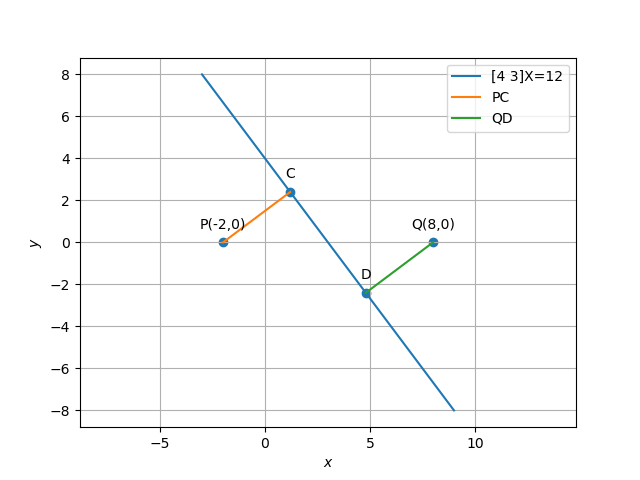
\includegraphics[width=\columnwidth]{chapters/11/10/3/5/figs/line2}
	\end{center}
\caption{}
\label{fig:11/10/3/5/Fig1}
\end{figure}


